%%%%%%%%%%%%%%%%%%%%%%%%%%%%%%%%%%%%%%%%%
% DOCUMENT CONFIGURATIONS
%%%%%%%%%%%%%%%%%%%%%%%%%%%%%%%%%%%%%%%%%

%----------------------------------------
% DOCUMENT TYPE
%----------------------------------------
\documentclass[
10pt, % Main document font size
a4paper, % Paper type, use 'letterpaper' for US Letter paper
oneside, % One page layout (no page indentation)
%twoside, % Two page layout (page indentation for binding and different headers)
%headinclude,footinclude, % Extra spacing for the header and footer
BCOR5mm, % Binding correction
]{scrartcl}
%
%
%----------------------------------------
% PACKAGES DOCUMENT CONFIGURATIONS
%----------------------------------------
\usepackage[square,numbers]{natbib} % bibliography with brackets and numbers
\usepackage[hidelinks]{hyperref} % black hyperlinks
\usepackage[toc]{appendix} % includes appendix in the TOC
\usepackage[nottoc,notlot,notlof]{tocbibind} % TOC
\usepackage{comment} % comment out some parts of the document
\usepackage{csquotes} % to insert quotes
\usepackage{color, colortbl} % defines colors and table colors
\usepackage[T1]{fontenc} % Use 8-bit encoding that has 256 glyphs
\usepackage[utf8]{inputenc} % Required for including letters with accents
\usepackage{graphicx} % Required for including images
\usepackage{enumitem} % Required for manipulating the whitespace between and within lists
%\usepackage{lipsum} % Used for inserting dummy 'Lorem ipsum' text into the template
\usepackage{subfig} % Required for creating figures with multiple parts (subfigures)
\usepackage{amsmath,amssymb,amsthm} % For including math equations, theorems, symbols, etc
\usepackage{varioref} % More descriptive referencing
\usepackage{authblk} % authors affiliation
\usepackage{tikz} % to generate DAGs
\usetikzlibrary{arrows.meta}
%
%
%----------------------------------------
% ADDITIONAL CONFIGURATIONS
%----------------------------------------
\graphicspath{{figures/}} % Set the default folder for images
%
\hyphenation{Fortran hy-phen-ation} % Specify custom hyphenation points in words with dashes where you would like hyphenation to occur, or alternatively, don't put any dashes in a word to stop hyphenation altogether
%
% THEOREM DEFINITION
\theoremstyle{definition} % Define theorem styles here based on the definition style (used for definitions and examples)
\newtheorem{definition}{Definition}
\theoremstyle{plain} % Define theorem styles here based on the plain style (used for theorems, lemmas, propositions)
\newtheorem{theorem}{Theorem}
\theoremstyle{remark} % Define theorem styles here based on the remark style (used for remarks and notes)
%
% define color for the rows of the table
\definecolor{gray}{gray}{0.95}
%
% HYPERLINKS
\hypersetup{
	%draft, % Uncomment to remove all links (useful for printing in black and white)
	colorlinks=true, breaklinks=true, bookmarks=true, bookmarksnumbered,
	urlcolor=webbrown, linkcolor=RoyalBlue, citecolor=webgreen, % Link colors
	pdftitle={}, % PDF title
	pdfauthor={\textcopyright}, % PDF Author
	pdfsubject={}, % PDF Subject
	pdfkeywords={}, % PDF Keywords
	pdfcreator={pdfLaTeX}, % PDF Creator
	pdfproducer={LaTeX with hyperref and ClassicThesis} % PDF producer
}
%
%
%%%%%%%%%%%%%%%%%%%%%%%%%%%%%%%%%%%%%%%%%
% DOCUMENT PRODUCTION
%%%%%%%%%%%%%%%%%%%%%%%%%%%%%%%%%%%%%%%%%
%
%----------------------------------------
% TITLE AND AUTHOR(S)
%----------------------------------------
%
\title{Speech intelligibility measurement} % The article title
\subtitle{A latent variable approach} % subtitle
\author[1]{Jose Rivera}
\affil[1]{ {\small Department of Training and Education Sciences, \authorcr
	University of Antwerp, Antwerp, Belgium  \authorcr
	E-mail: JoseManuel.RiveraEspejo@uantwerpen.be \authorcr
	(corresponding author) } }
\author[2]{Sven de Maeyer}
\affil[2]{ {\small Department of Training and Education Sciences, \authorcr
		University of Antwerp, Antwerp, Belgium  \authorcr
		E-mail: sven.demaeyer@uantwerpen.be \authorcr } }
\author[3]{Steven Gillis}
\affil[3]{ {\small Computational Linguistics, \& Psycholinguistics Research Centre \authorcr 
		University of Antwerp, Antwerp, Belgium \authorcr
		E-mail: steven.gillis@uantwerpen.be \authorcr } } 
%
\date{\today} % An optional date to appear under the author(s)
%
%
\begin{document}
%
%----------------------------------------
% TOC & LISTS OF FIGURES AND TABLES
%----------------------------------------
\maketitle % Print the title/author/date block
\setcounter{tocdepth}{3} % Set the depth of the table of contents to show sections and subsections only
%
\input 1_abstract
%
\newpage
\tableofcontents % Print the table of contents
%
\newpage
\listoffigures % Print the list of figures
\listoftables % Print the list of tables
%
%
%----------------------------------------
% DOCUMENT BODY
%----------------------------------------
\newpage
\input 2_introduction
\input 3_methods
\input 4_results
\input 5_discussion
\input 6_additionals
\appendix
%%%%%%%%%%%%%%%%%%%%%%%%%%%%%%%%
\section{Supplementary}
%%%%%%%%%%%%%%%%%%%%%%%%%%%%%%%%

%###############################
\subsection{Experiment details}
%###############################
%
%-------------------------------
\subsubsection{Transcription task} \label{appA:transcription}
%-------------------------------
%
The setting for the transcription task comprised the following steps \citep{Boonen_et_al_2020, Boonen_et_al_2021}:
%
\begin{enumerate} %\itemsep1pt
	\item the listener took a seat in front of a computer screen, located at the campus' computer laboratory.
	%
	\item the listener opened Qualtrics \cite{Qualtrics_2005} and select the transcription task.
	%
	\item the listener read two set of instructions presented on the computer screen about:
	\begin{enumerate}
		\item \textit{how to perform the task}, e.g. the listeners were instructed to write one \texttt{X} to replace an unintelligible word, part of an utterance, or a complete utterance,
		\item \textit{the aspects not to consider for the task}.
	\end{enumerate}
	%
	\item the listener hear the stimuli through high quality headphones, set at a comfortable volume.
	%
	\item the listener wrote the orthographic transcriptions of the utterances, in a free text field in the environment. 
	%
\end{enumerate}
%
%
%-------------------------------
\subsubsection{Entropy calculation} \label{appA:entropy} 
%-------------------------------
%
The outcome from the transcription task was obtained following a two step procedure \citep{Boonen_et_al_2021}. First, we aligned the participant's orthographic transcriptions, at the utterance level, in a column-like grid structure similar to the one presented in Table \ref{tab:align_example}. This step was repeated for every one of the $6400$ transcriptions. Lastly, we computed the entropy measure of the aligned transcriptions as in \citet{Shannon_1948}: 
%
\begin{equation} \label{eq:entropy}
	H = H(\pmb{p}) = \frac{-\sum_{i=1}^{n} p_{i} \cdot \log_{2}(p_{i})}{\log_{2}(N)}
\end{equation}
%
where $H$ is bounded in the continuum $[0,1]$, $n$ denotes the number of word occurrences within each utterance, $p_{i}$ the probability of such word occurrence, and $N$ the total number of aligned transcriptions per utterance.
%
\begin{comment}
under DoE literature, the design corresponds to $32$ experimental units with $10$ replicates each, making a total of $320$ experimental runs. Moreover, we register $20$ duplicates (transcriptions) for each run, making a total of $6400$ transcriptions.
\end{comment}
%
\begin{table}[h!]
	\centering
	\begin{tabular}{| c | ccccc | } 
		\hline
		Transcription & \multicolumn{5}{c |}{Utterance} \\ [0.5ex]
		\cline{2-6}
		number & 1 & 2 & 3 & 4 & 5 \\ [0.5ex] 
		\hline\hline
		1 & de & jongen & ziet & een & kikker \\ 
		& the & boy & see & a & frog \\ 
		\hline
		2 & de & jongen & ziet & de & [X] \\
		& the & boy & sees & the & [X] \\ 
		\hline
		3 & de & jongen & zag & [B] & kokkin \\
		& the & boy & saw & [B] & cook \\ 
		\hline
		4 & de & jongen & zag & geen & kikkers \\
		& the & boy & saw & no & frogs \\ 
		\hline
		5 & de & hond & zoekt & een & [X] \\
		& the & dog & searches & a & [X] \\ 
		\hline\hline
		Entropy & $0$ & $0.3109$ & $0.6555$ & $0.8277$ & $1$ \\
		\hline
		\multicolumn{4}{l}{\footnotesize{[B] = blank space, [X] = unidentifiable word}}
	\end{tabular}
	\caption[Alignment and entropy calculation]{Alignment and entropy calculation. Extracted from \citet{Boonen_et_al_2021}, and slightly modified with illustrative purposes.}
	\label{tab:align_example}
\end{table}
%

Entropy was used as a quantification of (dis)agreement between listeners' transcriptions, i.e. utterances yielding a high degree of agreement between transcribers were considered highly intelligible, and therefore registered a lower entropy $\left( H \rightarrow 0 \right)$. In contrast, utterances yielding a low degree of agreement were considered as exhibiting low intelligibility, and therefore registered a higher entropy $\left( H \rightarrow 1 \right)$ \citep{Boonen_et_al_2021, Faes_et_al_2021}. 

To exemplify relevant scenarios for the procedure, we generate the entropy for utterances $2$, $4$ and $5$ in Table \ref{tab:align_example}. To make the example easy to calculate, we assume our data consisted only of five transcriptions in total ($N=5$).

For the second utterance, we observe that four transcriptions identify it with the word \textit{jongen}, while the last with the word \textit{hond}. Therefore, we registered two word occurrences ($n=2$), with probabilities $\pmb{p} = (p_{1}, p_{2}) = (4/5, 1/5)$, and entropy measure equal to:
%
\begin{align*}
	H &= \frac{-\sum_{i=1}^{2} p_{i} \cdot \log_{2}(p_{i})}{\log_{2}(5)} \\
	%
	&= \frac{- \left[ 0.8 \log_{2}(0.8) + 0.2 \log_{2}(0.2) \right] }{\log_{2}(5)} \\
	%
	&\approx 0.3109
\end{align*} 
%
For the fourth utterance, we observe that two transcriptions identify it with the word \textit{een}, one with \textit{de}, one with \textit{geen}, and one with a blank space [B]. Notice the blank space was not expected in such position, therefore, it was considered as a different word occurrence. As a result, the scenario had four word occurrences ($n=4$), with probabilities $\pmb{p} = (p_{1}, p_{2}, p_{3}, p_{4}) = (2/5, 1/5, 1/5, 1/5)$, and entropy measure equal to:
%
\begin{align*}
	H &= \frac{-\sum_{i=1}^{4} p_{i} \cdot \log_{2}(p_{i})}{\log_{2}(5)} \\
	%
	&= \frac{- \left[ 0.4 \log_{2}(0.4) + 3 \cdot 0.2 \log_{2}(0.2) \right] }{\log_{2}(5)} \\
	%
	&\approx 0.8277
\end{align*} 
%
Finally, for the fifth utterance, we observe that all of the  transcriptions identify it with different words. Notice we consider the unidentifiable word [X] in the second transcription, as being different from the one in the last. This is done to avoid the artificial reduction of the entropy measure, as [X] values already indicate the lack of intelligibility of the word. Therefore, we registered five word occurrences ($n=5$), with probabilities $\pmb{p} = (p_{1}, \dots, p_{5}) = (1/5, \dots, 1/5)$, and entropy measure equal to:
%
\begin{align*}
	H &= \frac{-\sum_{i=1}^{5} p_{i} \cdot \log_{2}(p_{i})}{\log_{2}(5)} \\
	%
	&= \frac{- 5 \cdot 0.2 \log_{2}(0.2) }{\log_{2}(5)} \\
	%
	&= 1
\end{align*} 
%
%
%###############################
\subsection{Sampling bias}
%###############################
%
As it happens in most observational, and some experimental studies, ours can also be a potential victim of sampling bias. While stratifying on the selection variables can help to balance the samples, and even ``correct'' the estimates \cite{Cinelli_et_al_2021, Deffner_et_al_2022}, given the sample's selection and matching procedures, we cannot ensure the HI/CI nor the NH groups are representative of their respective populations. 

Nevertheless, we argue that by controlling for other relevant confounders, the qualitative results presented in this study holds. However, we cannot discard the presence of unobservable variables that could bias our results, and in that sense, inferences beyond this particular set of children must be taken with care.
%
%
%###############################
\subsection{Children characteristics} \label{appA:characteristics}
%###############################
%
Table \ref{tab:children_char} shows the detailed information of the sampled children. The referred table includes the variable used for the matching procedure, i.e. chronological age, while also additional variables thought to be relevant for our hypothesis. No other variables are included, as no known additional comorbidities, beside their hearing impairment, is suspected.

As it was mentioned in previous paragraphs, \textit{hearing age} is a composite measure, that tries to approximate the amount of time a child has been actively hearing and developing his(her) language. The variable is constructed combining the \textit{chronological age} for the NH group, and the \textit{device length of use} for the HI/CI group \citep{Faes_et_al_2021}.

Additionally, the table reports the child's etiology and their post-implant pure tone average (PTA). The etiology shows the cause of the children's hearing impairment, while PTA reports the child's subjective hearing sensitivity, aided and unaided by their hearing apparatus.
%
\begin{table}[h!]
	\centering
	\begin{tabular}{|c|ccccccc|} 
		\hline
		& Gender & Chronological age & Device length of use & Hearing age & Etiology & \multicolumn{2}{c |}{PTA (dB.)} \\[0.5ex]
		\cline{7-8}
		Child & & (y;m) & (y;m) & (y;m) & & unaided & aided \\[0.5ex] 
		\hline\hline
		& \multicolumn{7}{l |}{ \textbf{HI/CI children} } \\
		\rowcolor{gray}
		1 & female & 05;07 & 05;00 & 05;00 & Genetic & 120 & 19 \\
		2 & male & 06;04 & 05;09 & 05;09 & CMV & 106 & 23 \\
		\rowcolor{gray}
		3 & male & 06;07 & 05;10 & 05;10 & Genetic & 114 & 35 \\
		4 & female & 06;10 & 06;00 & 06;00 & Unknown & 120 & 20 \\ 
		\rowcolor{gray}
		5 & female & 07;00 & 06;03 & 06;03 & CMV & 115 & 25 \\ 
		6 & male & 07;00 & 05;08 & 05;08 & Genetic & 93 & 32 \\
		\rowcolor{gray}
		7 & female & 07;00 & 06;08 & 06;08 & Genetic & 117 & 17 \\
		8 & female & 07;00 & 05;05 & 05;05 & Unknown & 112 & 42 \\
		\rowcolor{gray}
		9 & male & 07;00 & 05;05 & 05;05 & CMV & 120 & 15 \\ 
		10 & female & 07;01 & 05;11 & 05;11 & Genetic & 120 & 35 \\		
		\rowcolor{gray}
		11 & male & 07;01 & 05;07 & 05;07 & Genetic & 113 & 42 \\
		12 & male & 07;02 & 06;05 & 06;05 & Genetic & 120 & 37 \\
		\rowcolor{gray}
		13 & male & 07;08 & 06;10 & 06;10 & CMV & 114 & 27 \\
		14 & male & 07;09 & 06;02 & 06;02 & CMV & 120 & 35 \\
		\rowcolor{gray}
		15 & male & 08;07 & 07;10 & 07;10 & CMV & 120 & 33 \\
		16 & male & 08;08 & 09;09 & 09;09 & Genetic & 95 & 27 \\
		& \multicolumn{7}{l |}{  }  \\

		& \multicolumn{7}{l |}{ \textbf{NH children} } \\	
		\rowcolor{gray}
		17 & female & 06;05 & n.a. & 06;05 & n.a. & n.a. & n.a.\\
		18 & female & 06;06 & n.a. & 06;06 & n.a. & n.a. & n.a.\\
		\rowcolor{gray}
		19 & female & 06;07 & n.a. & 06;07 & n.a. & n.a. & n.a.\\
		20 & female & 06;09 & n.a. & 06;09 & n.a. & n.a. & n.a.\\
		\rowcolor{gray}
		21 & female & 06;09 & n.a. & 06;09 & n.a. & n.a. & n.a. \\
		22 & male & 06;09 & n.a. & 06;09 & n.a. & n.a. & n.a.\\ 
		\rowcolor{gray}
		23 & male & 06;09 & n.a. & 06;09 & n.a. & n.a. & n.a.\\
		24 & male & 06;10 & n.a. & 06;10 & n.a. & n.a. & n.a.\\
		\rowcolor{gray}
		25 & female & 07;01 & n.a. & 07;01 & n.a. & n.a. & n.a.\\
		26 & male & 07;01 & n.a. & 07;01 & n.a. & n.a. & n.a.\\
		\rowcolor{gray}
		27 & male & 07;04 & n.a. & 07;04 & n.a. & n.a. & n.a.\\
		28 & female & 07;08 & n.a. & 07;08 & n.a. & n.a. & n.a.\\
		\rowcolor{gray}
		29 & male & 07;08 & n.a. & 07;08 & n.a. & n.a. & n.a.\\
		30 & female & 07;09 & n.a. & 07;09 & n.a. & n.a. & n.a.\\ 
		\rowcolor{gray}
		31 & female & 08;00 & n.a. & 08;00 & n.a. & n.a. & n.a.\\
		32 & female & 08;01 & n.a. & 08;01 & n.a. & n.a. & n.a.\\	 
		\hline
		\multicolumn{8}{l}{\footnotesize{(y;m) = (years;months)}} \\
		\multicolumn{8}{l}{\footnotesize{n.a. = not applicable / not available}} \\
	\end{tabular}
	\caption[Characteristics of selected children]{Characteristics of selected children.}
	\label{tab:children_char}
\end{table}
%
%
%###############################
\subsection{About speech intelligibility}
%###############################
%
Intelligible speech can be defined as the extent to which the elements in an speaker's acoustic signal, e.g. phonemes or words, can be correctly recovered by a listener \citep{Kent_et_al_1989, Whitehill_et_al_2004, vanHeuven_2008, Freeman_et_al_2017}. More specifically, in the context of the transcription task, speech intelligibility can be inferred from the extent a set of transcribers can identify the words contained in an utterance \cite{Boonen_et_al_2021}.

Therefore in this paper, through the implementation of our proposed model, \textit{speech intelligibility} is interpreted as a latent trait of individuals, which underlies the probability of observing a set of entropy replicates, that in turns, describes the ability of transcribers to identify the words in an utterance. Henceforth, statements such \textit{`speech intelligibility is influenced by'} can be read as \textit{`the probability of observing a set of entropy replicates for each individual in the sample is influenced by'}. 

Despite this practical approach, we want to emphasize we did our best to ensure the construct validity of our study, by ensuring the transcription task was well understood and appropriately performed by the transcribers.

We then expect speech intelligibility, as measured by our model, to reflect the (general unobserved) intelligibility of speech possessed by individuals, but do not deal with general epistemological considerations on the connection between the two.
%
%
%###############################
\subsection{DAG: factors influencing Intelligibility}
%###############################
%
Many factors have been shown to contribute to the success of spoken language development of children with CI, including: (1) audiology related factors, such as the age at implantation, the duration of device use, bilateral (or contralateral) cochlear implantation and the children’s preoperative and postoperative hearing levels; (2) child related factors, such as the cause of the hearing impairment (genetic, infections), gender, additional disabilities (mental retardation, speech motor problems); and (3) environmental factors, such as communication modality. An overview is provided in Boons, Brokx, Dhooge, Frijns, Peeraer, Vermeulen, Wouters, and van Wieringen, 2012, Fagan,
Eisenberg, and Johnson, 2020, Gillis, 2018 and Niparko, Tobey, Thal, Eisenberg, Wang,
Quittner, and Fink, 2010. A factor of particular importance here is age. Studies have shown
that chronological age is an important factor for intelligibility: as they grow older, children’s intelligibility increases irrespective of their hearing status (Grandon et al., 2020). But in the case of children with CI, age is a complicated factor, since it can not only refer to children’s chronological age (as is the case for children with NH), but also to the children’s so-called hearing age, which is the amount of time between the activation of their device and their chronological age. For instance, a child implanted at the age of 1;0 has a hearing age of two years at the age of 3;0. In addition, the age at implantation has been shown to play a critical role in children’s spoken language achievements. In general, earlier implantation appears to lead to better results than later implantation in several domains (Boons et al., 2012; Niparko et al., 2010). But the research findings with respect to the effect of the variable age on children with CI’s intelligibility are not unequivocal. In some studies, a significant effect of chronological age on children’s intelligibility was found (i.a., Flipsen, \& Colvard, 2006;
Grandon et al., 2020; Habib, Waltzman, Tajudeen, \& Svirsky, 2010) but not in others (e.g.,
Khwaileh, \& Flipsen, 2010). Hearing age was found to be a significant predictor of intelligibility by i.a., Flipsen and Colvard (2006), but hearing age was not always considered as a predictor. Age at implantation predicted children’s intelligibility in a considerable number of studies (i.a., Grandon et al., 2020; Habib et al., 2010; Montag, AuBuchon, Pisoni, \& Kronenberger, 2014; Svirsky, Chin, \& Jester, 2007) but this was not the case in other studies (i.a., Flipsen, \& Colvard, 2006; Khwaileh, \& Flipsen, 2010). Nevertheless, a general finding appears to be that earlier implantation leads to better results in speech and language development and in intelligibility. At present there is consistent evidence that implantation in the first two years of life leads to consistently better results in spoken language development in comparison to later implantation, and even (inconclusive) evidence for even better outcomes of implantation in the first year of life (Bruijnzeel et al., 2016; Dettman et al., 2016).



%###############################
\subsection{Model details}
%###############################

%-------------------------------
\subsubsection{Definition}
%-------------------------------
%
Previous research already used hierarchical models with the replicated entropy measures as outcomes \citep{Boonen_et_al_2021, Faes_et_al_2021}. Hierarchical models are powerful to control for heterogeneity in the data, and also to avoid pre-aggregating procedures that could be pernicious for a proper statistical inference \citep{McElreath_2020}. 

These claims are easier to understand using a though experiment within our research. Consider we have two children with the same mean entropy, but the second child shows more variability across the $10$ utterances than the first. It is clear that the average entropy measure informs about the child's average SI, indicating that both children have similar level. However, the entropy's heterogeneity across the $10$ utterances also informs about the child's SI, as a higher variability imply transcribers agreed less about the second child's intelligibility.

The intuition derived from the previous though experiment is similar to the one presented in \citet{Boonen_et_al_2021}, and it is what justify our use of a hierarchical model. More specifically, we will use a Hierarchical (Mixed) Beta Regression model \citep{Figueroa-Zuniga_et_al_2013}, for which we argue, its implementation is rather trivial under the bayesian framework, and we present it in the following lines.

First, figure \ref{fig:entropy_ME} depicts the DAG representation of the model. For the measurement error part, section \ref{ss_sect:outcome} reveals the (observed) entropy replicates $H^{O}_{ik}$ can represent multiple realizations of a child's \textit{true} entropy $H^{T}_{i}$, measured with error $e_i$. As a result, we can say the $k$'th entropy measure is nested within the $i$'th child, where $k=1, \dots, K$, $i=1, \dots, I$, $K = 10$ utterances, and $I = 32$ children.

Second, for the hypothesis part, we can say the child's \textit{true} entropy $H^{T}_{i}$ is inversely explained by the child's speech intelligibility index $SI_{i}$, and in turn, the latter by a set of covariates. Notice from Figure \ref{fig:entropy_ME}, we propose two sets of models. The model in panel (a) use hearing status ($HS_{i}$) and hearing age ($A_{i}$) as covariates. The use of hearing status is justified as we are interested in comparing SI among groups, defined by the children's hearing characteristics (NH, HI/CI, and HI/HA). On the other hand, we expect hearing age\footnote{see section \ref{s_sect:children} to know how the variable is defined.} and its interaction with hearing status, to also have an effect on the SI index, as previous evidence have shown the speech of HI children gradually approximate that of NH children \citep{Boonen_et_al_2019}.

Notice the model depicted in panel (a) is interested on (what we can call) \textit{total effects}, i.e. the effects of the hearing characteristics, not independent from the effects of the hearing apparatus (cochlear implant or hearing aid). This is important to understand for two reasons. Since a hearing apparatus is fitted onto a child depending on aspects such as the locus and severity of his(her) hearing impairment \citep{Korver_et_al_2017}: (1) such specific children's characteristics could confound the (beneficial) effects of using specific hearing apparatuses, while (2) because children are selected from a convenient sample, not representative of their respective populations (see section \ref{s_sect:children}), the need to control for such characteristics is paramount, if we seek to obtain effects that can generalize better and beyond our sample\footnote{follow the \textit{notes} folder, to see a graphical though experiment.}.

Considering the previous, we propose the model depicted in panel (b), where we control for the possible confounding variables etiology ($E_{i}$), \textcolor{blue}{as a proxy of locus}, and unaided PTA ($PTA_{i}$), as a proxy for hearing impairment severity. In that sense, the model would estimate (what we can call) the \textit{direct effects} of the hearing apparatus, independent of the children's characteristics.

Lastly, we proceed to use probabilistic programming to declare the algebraic structure of our models. Given the panel (a) model is nested within the panel (b) model, we declare only the model structure for the latter:
%
\begin{align}
	%
	H^{O}_{bik} & \sim \text{BetaProp} \left( P_{bi}, M_{ik} \right) \\ 
	%
	P_{bi} &= \alpha_{b} + H^{T}_{i} \\
	%
	H^{T}_{i} &= \text{logit}^{-1}( -SI_{i} ) \\
	%
	SI_{i} & = a_{i} + \alpha + \alpha_{E[i],HS[i]} + \beta_{A, HS[i]} (A_{i} - \bar{A}) + \beta_{P} PTA_{i} \\ 
	%
\end{align}
%
where $\text{logit}(x) = \log \left[ x / ( 1 - x ) \right]$, and $\text{logit}^{-1}(x) = \exp(x) / ( 1 + \exp(x) ) $. Additionally, a $\text{BetaProp}(\mu, \theta)$ distribution is equal to a $\text{Beta}(\alpha, \beta)$ distribution, with $\alpha=\mu \theta$, $\beta=(1-\mu)\theta$. For our purposes, $\mu = H^{T}_{i}$ and $\theta = M_{i}$, the latter denoting the ``sample size" of the distribution. Moreover, $a_{i}$ denote the children's random effects, $\alpha$ the fixed effects' intercept, $\alpha_{HS[i]}$ and $\beta_{A, HS[i]}$ the intercept and slope of ``hearing age" per hearing status group, $\alpha_{E[i]}$ the intercept per etiology group, and $\beta_{P}$ the slope for the standardized PTA levels. 

Three important things need to be noticed from the previous algebraic structure. First, all the parameters are estimated in the logit scale and centered at $PTA_{i}=0$ and $\bar{A}$, which denotes the minimum hearing age in the sample. Second, instead of a latent measurement error $U_{ik}$, we use the latent ``sample size" parameter $M_{ik}$ to model the heterogeneity/variability of the duplicate entropies. This effectively works as a measurement error model for the replicates, as the parameter defines the shape of the distribution. Third, if we do not consider etiology and PTA values in equation (4), we obtain the panel (a) model.
%
\begin{figure}
	\centering
	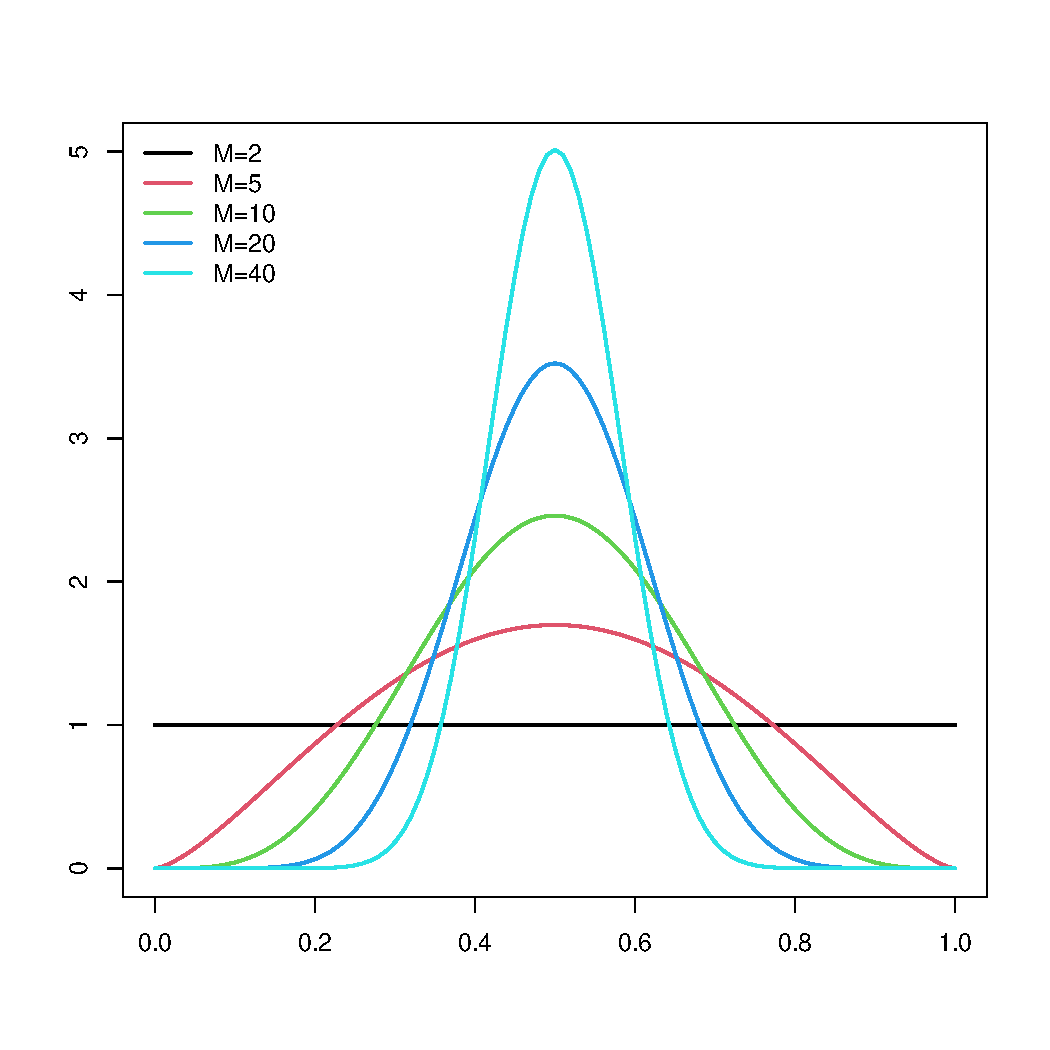
\includegraphics[width=0.5\linewidth]{BetaProp_dist.pdf}
	\caption[Variability in a Beta-Proportional distribution]{Variability in a Beta-Proportional distribution.}
	\label{fig:BetaProp}
\end{figure}
%
%
%-------------------------------
\subsubsection{Priors}
%-------------------------------
%
\begin{align}
	%
	M_{i} & \sim \text{LN}( \mu_{M}, \sigma_{M}) \\
	%
	a_{i} & \sim \text{N}(\mu_{a}, \sigma_{a}) \\
	%
	\alpha & \sim \text{N}(0, 0.3) \\
	%
	\alpha_{HS[i]} & \sim \text{N}(0, 0.3) \\
	%
	\beta_{A, HS[i]} & \sim \text{N}(0 , 0.3) \\
	%
	\alpha_{E[i]} & \sim \text{N}(0, 0.5) \\
	%
	\beta_{P} & \sim \text{N}(0, 0.3) \\
	%
	\mu_{M} & \sim \text{N}(0, 5) \\
	%
	\sigma_{M} & \sim \text{Exp}(1) \\
	%
	\mu_{a} & \sim \text{N}(0, 0.5) \\
	%
	\sigma_{a} & \sim \text{Exp}(1)\\
	%
\end{align}
Third, we use mildly informative priors to state our uncertainty regarding the direction and magnitude of the effects\footnote{see \citet{Rivera_2021} (p. 18-19) for an intuition on prior elicitation.}. 
\begin{figure}
	\centering
	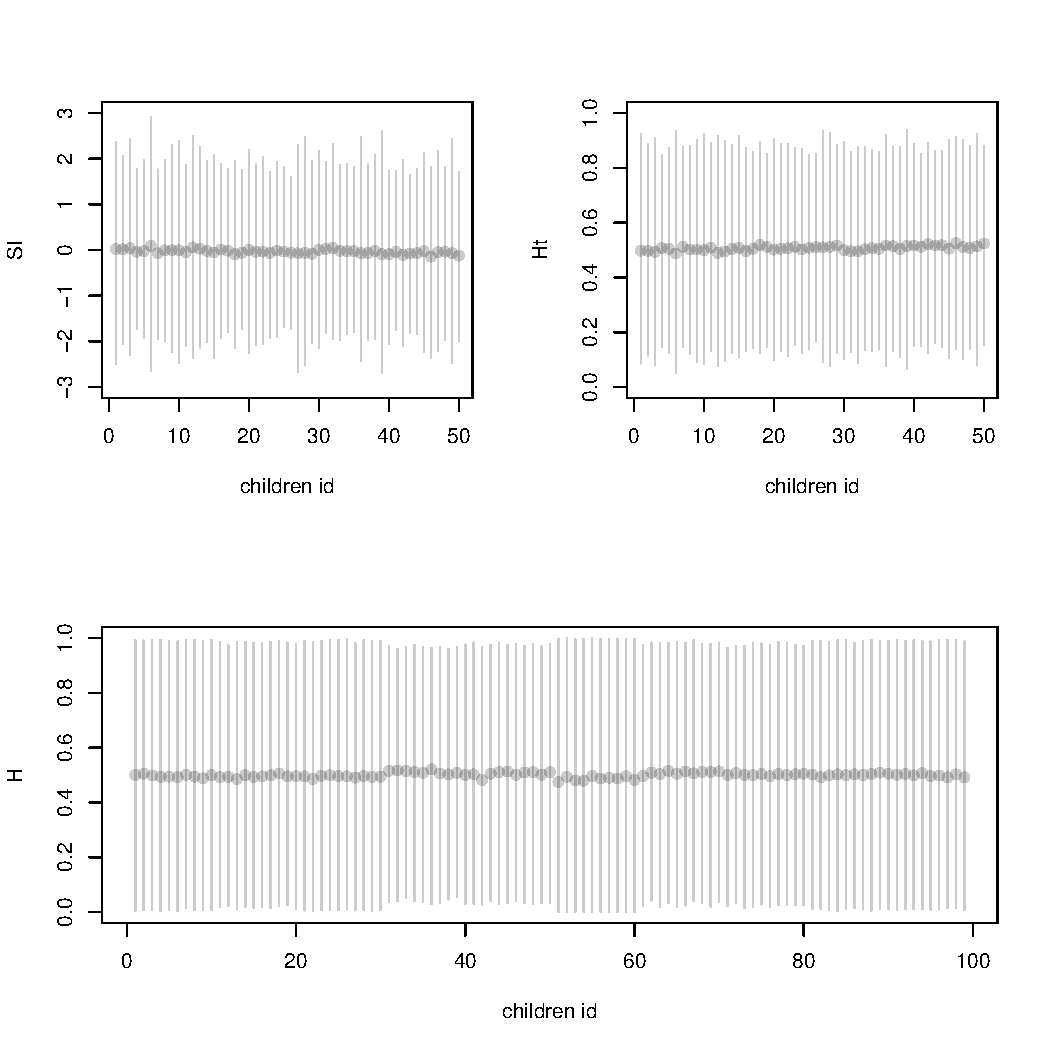
\includegraphics[width=0.6\linewidth]{prior_predictive.pdf}
	\caption[Prior distribution implications]{Prior distribution implications. Speech intelligibility, ``true'' entropy and observed entropy scales.}
	\label{fig:priors}
\end{figure}
%
%
%-------------------------------
\subsubsection{Estimation}
%-------------------------------
The models proposed in sections \ref{s_sect:evaluation} and \ref{s_sect:models} will be estimated under the Bayesian framework\footnote{see \citet{Rivera_2021} (p. 11-13, 15-27) for a detailed description of its benefits and shortcomings.}. More specifically, we will use the No-U-Turn Hamiltonian Monte Carlo algorithm (No-U-Turn HMC) \citep{Betancourt_et_al_2013, Duane_et_al_1987, Hoffman_et_al_2014, Neal_2012}. \texttt{Stan} \citep{Stan_2020} will be the software package that will provide us with the No-U-Turn HMC machinery, while \texttt{R} \citep{R_2015} and its integration packages \citep{RStan_2020}, the software that will allow us to analyze its outputs.
%
%
%-------------------------------
\subsubsection{Pre-processing} \label{ss_sect:preproc}
%-------------------------------
%
Besides the exclusion of corrupted observations, e.g. no available rating, no other experimental run nor duplicate was eliminated before the modeling process. This decision departs from what it is observed in previous research, e.g. \citet{Boonen_et_al_2020} decided to eliminate "outlying" observations based on misfit analysis \citep{Lesterhuis_2018}, while \citet{vanDaal_2020} and \citet{Boonen_et_al_2021} did the same based on univariate outlier analysis. 

For the case of misfit analysis, we argue that such procedures cannot be used without caution. The literature points out that in the context of CJ, these statistics are always relative, i.e. they depend on other stimulus and judges included in the assessment \citep{Pollitt_2012a, Pollitt_2012b}. Moreover, they have been proven to be less sensitive, as they are calculated with a low number of judgments per representation \citep{Pollitt_2012a}. 

On the other hand, for the case of univariate outlier analysis, we argue that outlying observations are interesting cases to analyze \citep{McElreath_2020}, and usually they cannot be identified properly outside the context of a full model \citep{McElreath_2020}, i.e. what can behave as an outlier based on a univariate analysis, can behave as expected under the appropriate model. 

Considering the previous, if we still manage to identify outlying observations within the context of the proposed models (see Section \ref{s_sect:models}), the researcher would rather make the model robust against their influence, playing on the strengths of the bayesian framework, than to eliminate the observations. 
%
%
%-------------------------------
\subsubsection{Simulation}
%-------------------------------
Preliminary to the data collection, we simulated data in silico to test the models and inform data collection procedure. The simulation code is available in the GitHub repository. Several functional correlation between age and knowledge have been simulated, and the model used in the analysis - which includes age as a ordinal categorical predictor of knowledge with monotonically increasing effect - has been able to recover the different shapes. Causal effect of activities, family composition and schooling have been simulated and tested.

The simulated data have been used -albeit in a previous version- to estimate the minimum number of interviewees necessary to recover the parameter values. If individuals were to name a maximum of 300 items in the freelist, 50 interviewees would have been suffcient to obtain reliable estimates of the parameters. Given that data collection in vivo is much less regular and less controllable than in silico, we roughly doubled the number of interviewees and that of questions.


%-------------------------------
\subsubsection{Model selection}
%-------------------------------
%
Following the successful and comprehensive analysis in \citet{vanDaal_2020} and \citet{Lesterhuis_2018}, the current research will also use the Information-Theoretic Approach (ITA) \citep{Anderson_2008, Chamberlain_1965} for the selection of competing models. The approach considers three steps: (1) state our hypothesis into statistical models, (2) select among competing models, and (3) make inferences based on one or multiple models.

First, for the translation of our working hypotheses into statistical models, we will use Directed Acyclic Graphs (DAG) and probabilistic programming \citep{Jaynes_2003}. A DAG is the simplest representation of a Graphical Causal Model (GCM), a heuristic model that contains information not purely statistical, but unlike a detailed statistical model, it allow us to deduce which variable relationships can provide valid causal inferences \citep{Hernan_et_al_2020, McElreath_2020}. In summary, a DAG is a reasonable way to state our hypothesis, and make our assumption more transparent. However, abide by the \textit{no-free lunch} rule, the causal inferences produced under the DAG will only be valid if the assumed DAG is correct. In contrast, the probabilistic programming will serve as the algebraic formalist to define our statistical models.

Second, to select among competing models, we will use the Widely Applicable Information Criterion (WAIC) \citep{Watanabe_2013}, and the Pareto-smoothed importance sampling cross-validation (PSIS) \citep{Vehtari_et_al_2021}\footnote{\citet{vanDaal_2020} used the Akaike’s Information Criterion (AIC) \citep{Akaike_1974} with similar purposes.}. Two reasons justify our decision. First, both criteria allow us to embrace the full flexibility and information of our bayesian implementation (outlined in Section \ref{s_sect:models}). Last, and more important, both criteria provide us with the best approximations for the out-of-sample (cross-validated) deviance \citep{McElreath_2020}. The deviance is the best approximation for the Kullback-Liebler (KL) divergence \citep{Kullback_et_al_1951}, i.e. a measure of how far a model is from describing the \textit{true} distribution of our data. \citet{McElreath_2020} points out that is a rather benign characteristic of the model's selection procedure that we do not need the KL divergence's absolute value, as the \textit{true} distribution of our data is not available (otherwise, we would not need a statistical model). But rather, using the difference in deviance between competing models, we can measure which model is the farthest from \textit{perfect (predictive) accuracy} for our data\footnote{see \citet{McElreath_2020} (p. 202-211) for the intuition and detailed derivation of the argument.}.

Finally, considering the evidence provided by the previous step, we proceed to make inferences based on one or multiple models.
%
%
%----------------------------------------
%	BIBLIOGRAPHY
%----------------------------------------
%
\renewcommand{\refname}{\spacedlowsmallcaps{References}} % For modifying the bibliography heading
\newpage
\bibliographystyle{dcu}
\bibliography{bibliography.bib}
%
%
\end{document}